%! Author = melek
%! Date = 29.12.2022

% Preamble
\documentclass[11pt]{article}

% Packages
\usepackage{amsmath}
\usepackage{graphicx}
\graphicspath{ {../images/} }

\title{Assignment 2: Policy Gradients}
\author{huseyinabanox@gmail.com}
\date{January 2023}

% Document
\begin{document}

    \maketitle

    \section{Small-Scale Experiments}

    \subsection{Experiment 1}




    Reward-to-go estimator performs better.
    Advantage standardization difference is not statistically significant.


    \hspace*{-0.5in}
    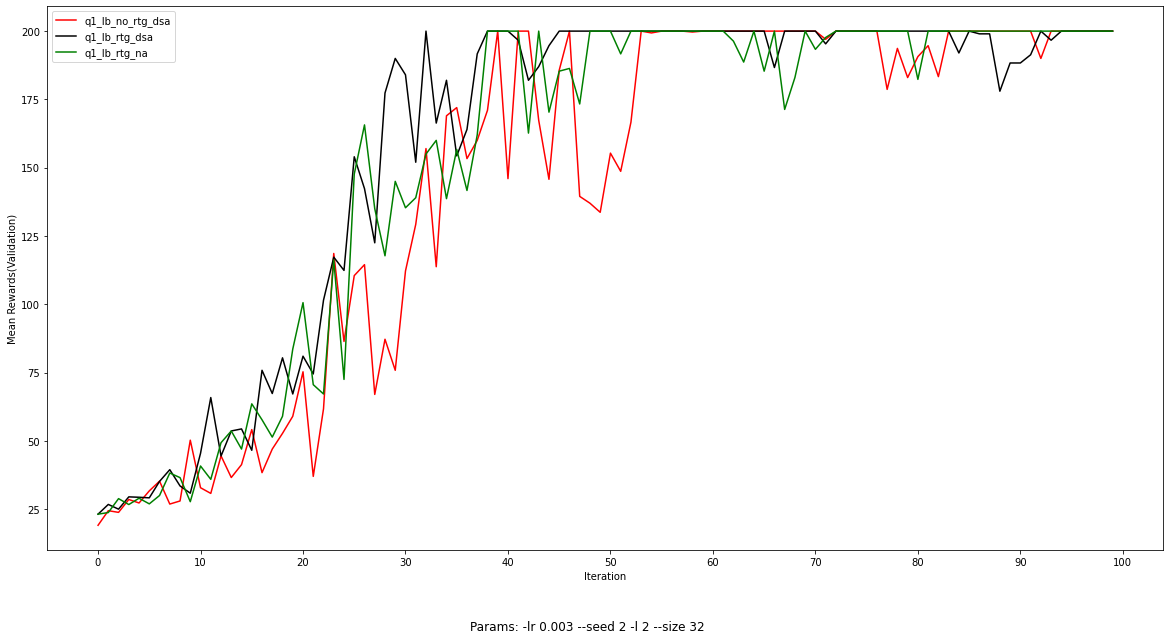
\includegraphics[scale=0.35]{q1/q1_lb_plot}

    Reward-to-go estimator performs better.
    Advantage standardization difference is not statistically significant.
    Increasing the batch size helps the trajectory-centric algorithm converge with fewer iterations.


    \subsection{Experiment 2}

    \hspace*{-0.5in}
    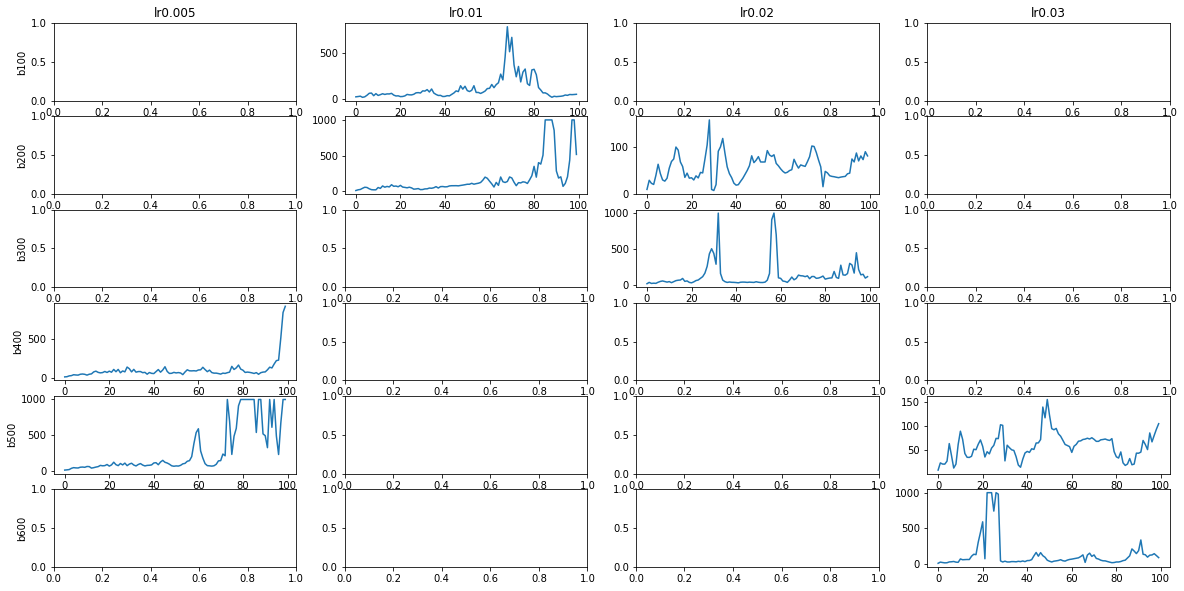
\includegraphics[scale=0.35]{q2/q2_grid_plot}

    A grid search with default parameters shows that it is possible to reach the target reward of 1000 with learning rate 0.01 and batch size 200 or with learning rate 0.02 and batch size 300.
    The first options seems to be more stable.

    Please note that the figure tries to show the boundary in hyperparameter space.
    In each column the first chart indicates the largest learning rate and smallest batch size that fails to reach 1000.
    In each column the second chart indicates the largest learning rate and smallest batch size that succeeds in reaching 1000.

    \subsection{Experiment 3}

    \hspace*{-0.5in}
    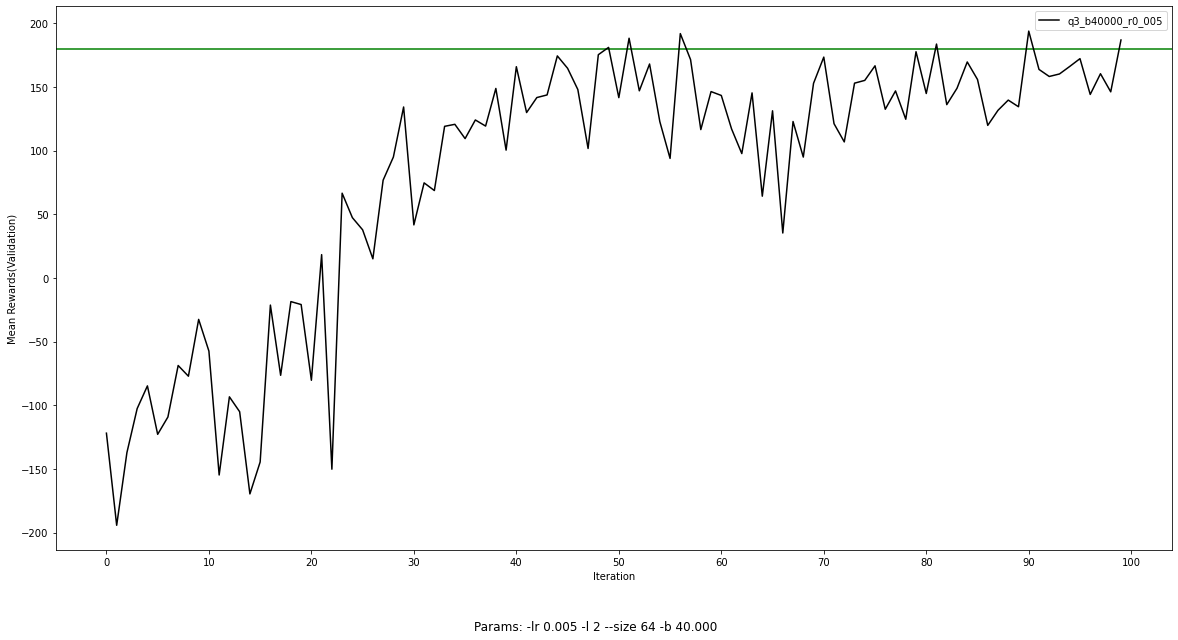
\includegraphics[scale=0.35]{q3/q3_b40000_r0.005_mean_rewards}

    \subsection{Experiment 4}

    A trial and error search is run on hyperparameter space.
    Learning rate 0.02 and batch size 50K are found to be best performing.

    \hspace*{-0.75in}
    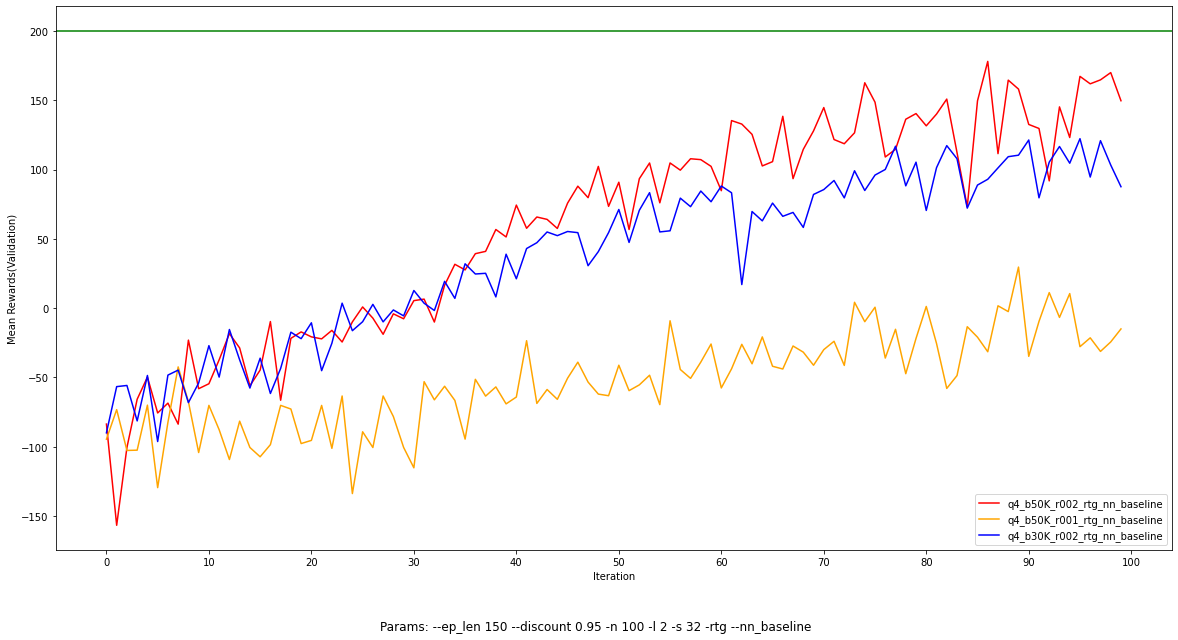
\includegraphics[scale=0.35]{q4/q4_parameter_comparison}

    The chart above shows evaluation results by iteration for different parameter sets.

    Bigger batch size is better.
    It reduces variance and speeds up learning.

    Bigger learning rate is better.
    It speeds up learning.
    If learning rate is too large, it may cause converging to a local minimum or divergence.

    While doing trial and error, largest possible values are selected at first.
    Then a smaller learning rate configuration is tested.
    Then a smaller batch size configuration is tested.
    Both configurations are found to perform worse than the first test.

    \hspace*{-0.75in}
    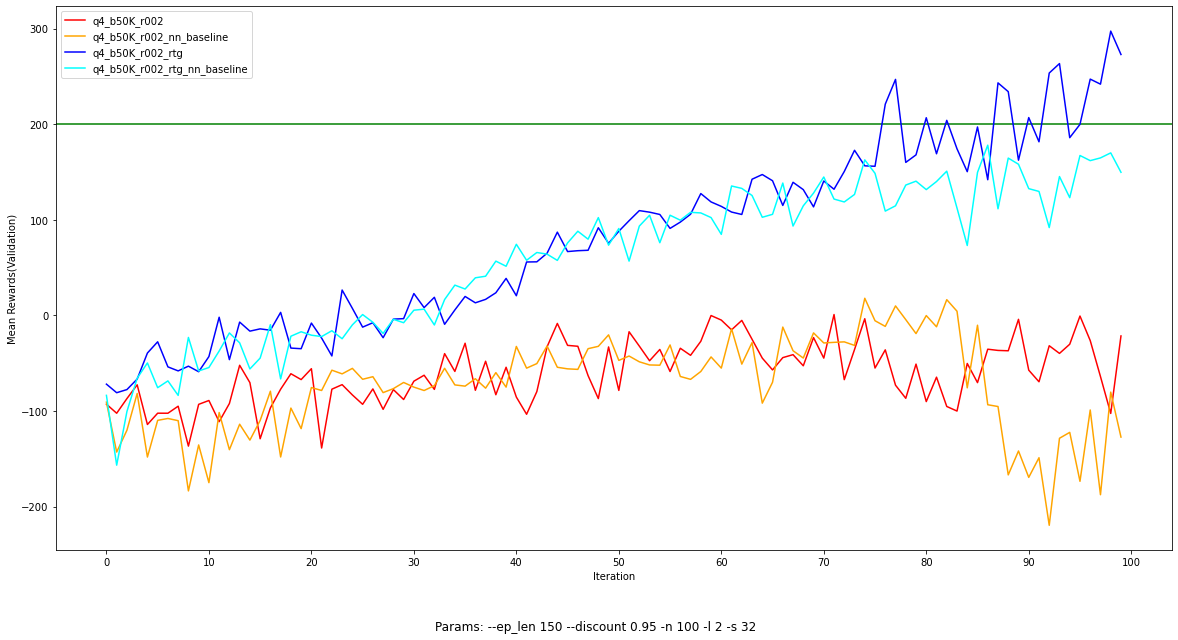
\includegraphics[scale=0.35]{q4/q4_rtg_baseline_comparison}

    The chart above shows performance for different reward-to-go and baseline parameter configurations.
    Reward-to-go always performs better.
    However, the one with baseline was expected to perform better with less variance which seems not to be the case.
    It is not clear whether this is bacause of random initialization or implementation issues.


    \subsection{Experiment 5}

    First chart shows lambda 1.0 and vanilla neural network baseline estimator.
    Noise parameter is not added to the vanilla estimator.
    They are somewhat similar which is expected.

    \hspace*{-0.75in}
    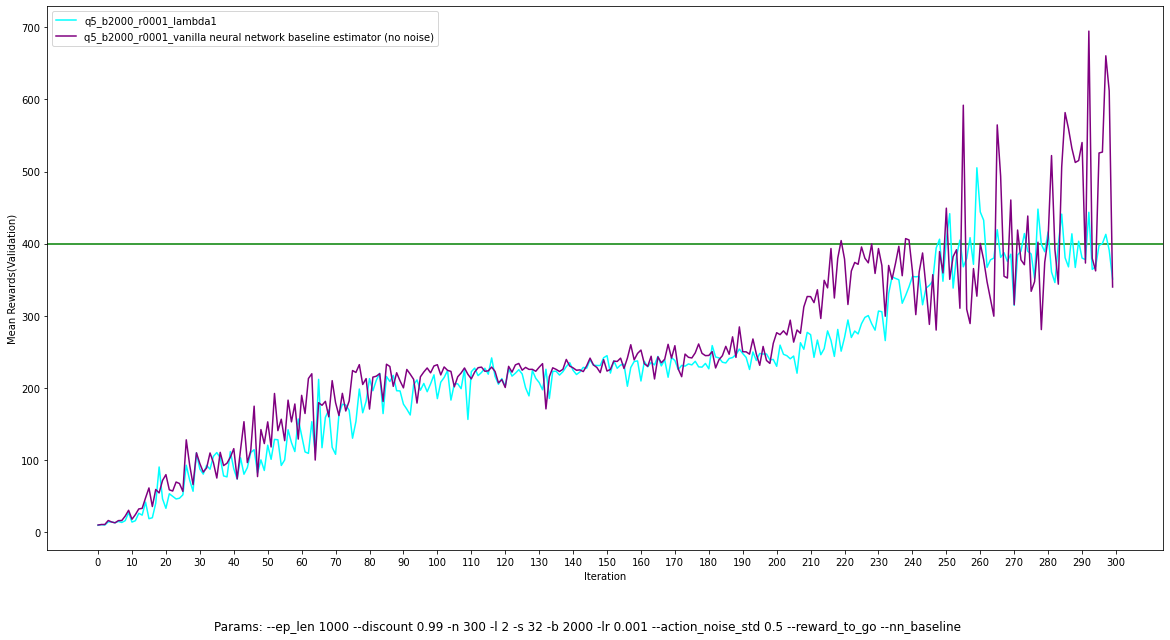
\includegraphics[scale=0.35]{q5/q5_lambda1_vs_vanilla}

    The following chart shows learning curves for different lambda values.

    \hspace*{-0.75in}
    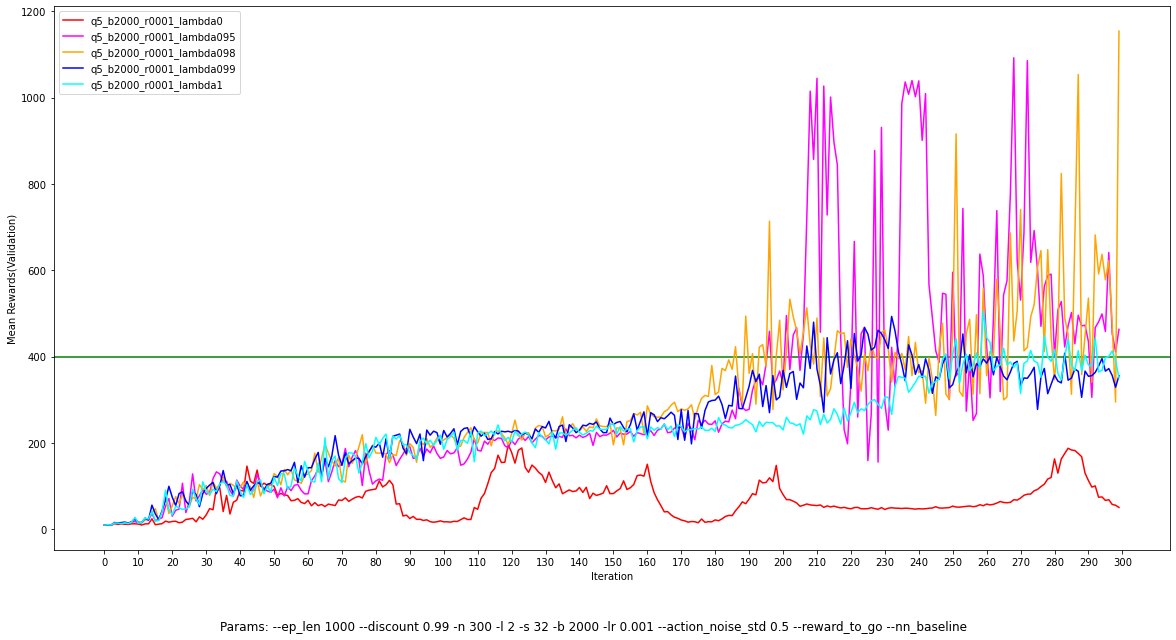
\includegraphics[scale=0.35]{q5/q5_lambda_compare}

    As lambda moves away from 1, variance grows.
    The best performance is obtained when the lambda is set to 1.0.
    The second best is lambda 0.99.
    lambda value 0.99 learns faster, it reaches the target mean reward more quickly.
    However, it fluctuates a lot when compared to lambda value 1.0.

    The lower the lambda parameter, the algorithm cares less about the future and this behaviour adds to variance.
    When lambda is zero, the algorithm onl cares about the current step value.
    In this case the performance is the worst.
    When lambda is set to 1, the algorithm cares about future rewards as much as the current reward and the performance is the best.
\end{document}